%%%%%%%%%
\begin{figure*}
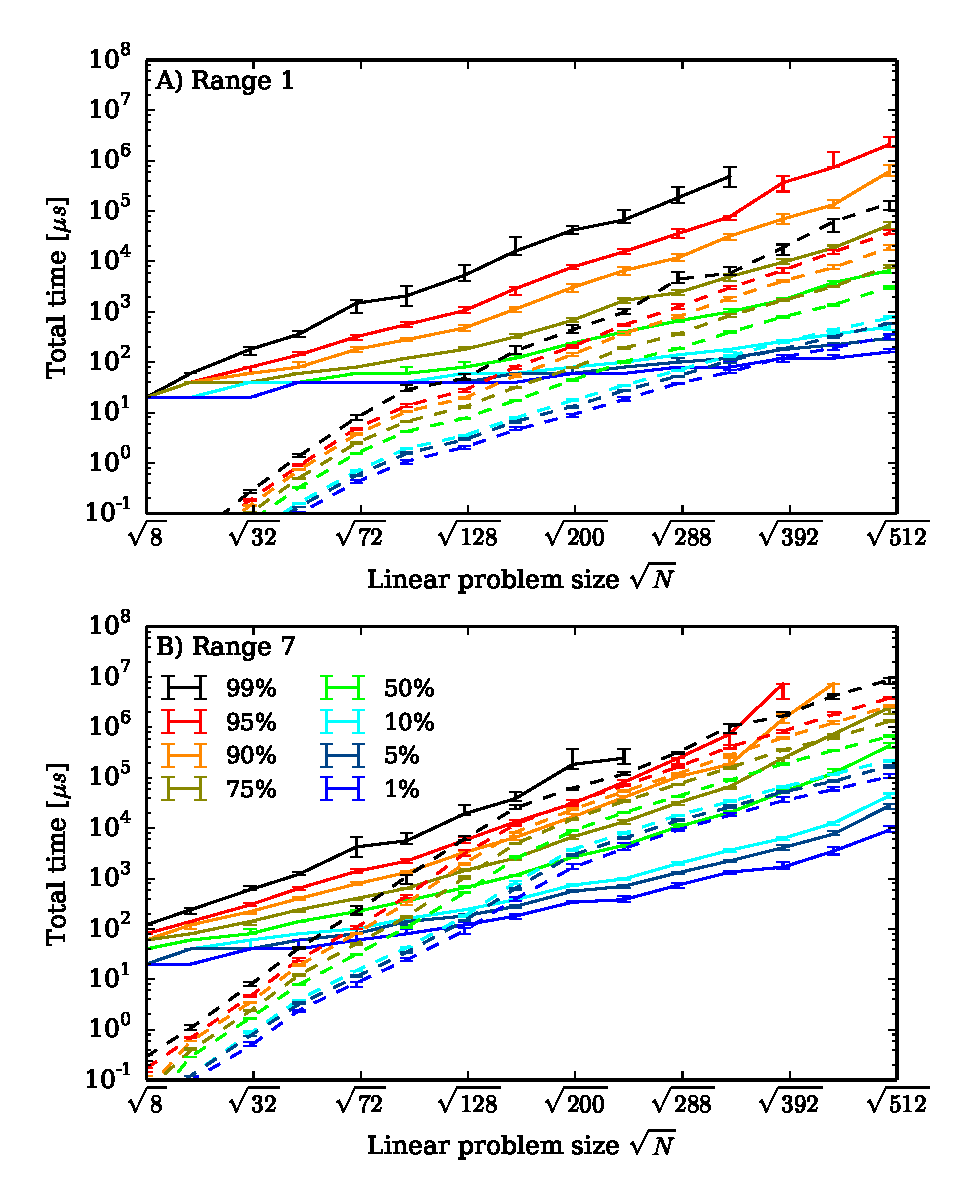
\includegraphics[width=1\columnwidth]{fig03.pdf} 
\label{fig:scalingraw7}
\caption{{\bf Scaling of time to solution for the ranges $r=1$ (panel A) and $r=7$ (panel B).} Shown is the scaling of the pure annealing time to find the ground state at least once with a probability $p=0.99$ for various quantiles of hardness, for simulated annealing (SA, dashed) and the DW2 (solid). 
%The SA data was obtained by running the simulations at an optimized annealing time for each problem size. The DW2 a nnealing time of $20\mu s$ is the shortest possible. 
The solid lines terminate for the highest quantiles because the DW2 did not solve the hardest instances for large problem sizes within the maximum number of repetitions (at least 32000) of the annealing we performed. 
}
\label{fig:scalingraw}
\end{figure*}
%%%%%%%%%

